\documentclass[11pt]{article}

\usepackage[letterpaper,margin=1in]{geometry}
\usepackage[T1]{fontenc}
\usepackage{lmodern}
\usepackage{microtype}
\usepackage{amsmath,amssymb,amsthm}
\usepackage{graphicx}
\usepackage{booktabs}
\usepackage[font=small,labelfont=bf]{caption}
\usepackage{xcolor}
\usepackage[colorlinks=true,linkcolor=blue!50!black,citecolor=blue!50!black,urlcolor=blue!50!black]{hyperref}

\newcommand{\R}{\mathbb{R}}
\newcommand{\Prob}{\mathbb{P}}
\DeclareMathOperator{\sgn}{sgn}

\title{Noise and the Fractal Convergence Boundary\\ of Gradient Descent with Large Step Sizes}
\author{Arav Rawat\\[2pt]
\small Granada Hills Charter High School\\
\small \href{mailto:aravrawatcollege@gmail.com}{\texttt{aravrawatcollege@gmail.com}}}
\date{October 2026}

\begin{document}
\maketitle

\begin{abstract}
\noindent
Liang and Mont\'ufar showed that gradient descent on regularized scalar factorization, run with a step size close to the critical value, has a convergence region with a fractal boundary. We study numerically how this boundary responds to three kinds of noise: a randomized step size, stochastic gradient descent on a two-sample finite sum, and isotropic Gaussian gradient noise. Because a single noisy trajectory per initialization yields a map dominated by sampling fluctuations, we work instead with outcome probabilities estimated from many independent runs. We find that small noise blurs the boundary into a band of uncertain outcomes whose area grows as a power law in the noise level, while the location of the boundary changes very little. Which minimizer is selected is more sensitive to noise than whether the iteration converges. At larger noise levels the three noise models behave differently: a randomized step size enlarges the convergence region, SGD loses its minimizers once the noise exceeds $y-\lambda$, and isotropic noise makes the selected minimizer essentially random. Code and data are available at \url{https://github.com/lnxv/fractal-convergence-noise}.
\end{abstract}

\section{Introduction}

For gradient descent with a large step size, the set of initializations from which the iteration converges can have a fractal boundary. This has been observed for neural network training by Sohl-Dickstein~\cite{sohldickstein2024}, and Liang and Mont\'ufar~\cite{liang2026} proved results of this type for the simplest nontrivial model, regularized scalar factorization
\begin{equation}\label{eq:loss}
  L(u,v) = \tfrac12 (uv-y)^2 + \tfrac{\lambda}{2}\,(u^2+v^2), \qquad (u,v)\in\R^2,
\end{equation}
with $0<\lambda<y$. Gradient descent on~\eqref{eq:loss} with step size $\eta$ has two minimizers $\pm(m,m)$, where $m=\sqrt{y-\lambda}$. In~\cite{liang2026} the authors identify a critical step size above which GD fails to converge from almost every initialization, and show that close to this value the convergence region has a fractal boundary; for $\eta=1$, $\lambda=0.2$ and $y=0.5$ they estimate a box-counting dimension of $1.249$ for its projection onto the coordinates $(uv,\,u^2+v^2)$.

Gradient descent is rarely run without noise in practice. The aim of this note is to ask whether a small amount of noise preserves the fractal boundary, blurs it, or changes it qualitatively, and what happens as the noise level increases. Our approach follows the probability-basin method of Nieto, Seoane and Sanju\'an~\cite{nieto2021}, who studied final-state sensitivity in noisy chaotic scattering, and compares it with the uncertainty exponent of Grebogi, McDonald, Ott and Yorke~\cite{grebogi1983} for the deterministic iteration.

\section{Setup}

Throughout we fix $\eta=1$, $\lambda=0.2$ and $y=0.5$, the setting of Figure~3 in~\cite{liang2026}. We consider three perturbations of the gradient step $(u,v)\mapsto (u,v)-\eta\nabla L(u,v)$:
\begin{enumerate}
  \item \emph{Step noise.} The step size is $\eta_t=\eta(1+\sigma\xi_t)$ with $\xi_t\sim U(-1,1)$ independent. The minimizers remain fixed points.
  \item \emph{SGD.} The loss is written as the finite sum $L=\frac12(L_++L_-)$ over two data points $y\pm\sigma$, where $L_\pm$ is~\eqref{eq:loss} with $y$ replaced by $y\pm\sigma$, and one of the two is chosen uniformly at random at each step. The minimizers of $L$ are unchanged and the gradient noise depends on the state.
  \item \emph{Additive noise.} $\nabla L$ is replaced by $\nabla L+\sigma\zeta_t$ with $\zeta_t\sim N(0,I_2)$ independent.
\end{enumerate}
A run \emph{escapes} if $\max(|u_t|,|v_t|)$ exceeds $10^8$ within $T=200$ steps; otherwise it \emph{survives}, and its final state is classified as close to $+(m,m)$, close to $-(m,m)$, or neither.

For each initialization $(u_0,v_0)$ we estimate from $n$ independent runs the probability of survival and the probabilities $p_\pm$ of ending close to each minimizer. We call an initialization \emph{uncertain for escape} if $0.1<\Prob(\text{survive})<0.9$, and \emph{uncertain for selection} if it usually survives but $0.1<p_+/(p_++p_-)<0.9$. The fractions of such initializations in a region are our main quantities. Near the boundary we use two windows, $W_1=[2,2.7]\times[-0.3,0.3]$ and $W_2=[1.7,2.3]\times[0.5,1.1]$, sampled on $101\times101$ grids with $n=96$; over the whole domain $[-4,4]^2$ we use a $161\times161$ grid with $n=32$.

As a reference for the deterministic iteration, we compute the uncertainty exponent~\cite{grebogi1983}. For $40{,}000$ random points in each window, we test whether a perturbation of size $\varepsilon$ changes the outcome. The fraction $f(\varepsilon)$ of such points scales as $\varepsilon^{\alpha}$ with $\alpha=2-D$, where $D$ is the dimension of the boundary.

\section{Reproducing the deterministic results}

Before adding noise we checked that the deterministic phenomenon is recovered (Figure~\ref{fig:repro}). The convergence region on $[-4,4]^2$ agrees with Figure~3 of~\cite{liang2026}. Applying box counting to the boundary of the projected planar map of their Proposition~3 gives a dimension of $1.249$ ($R^2=0.9966$), matching the reported value. For the critical step size of their Theorem~1, gradient descent converged from all of $20{,}000$ random initializations when $\eta$ was $3\%$ or $10\%$ below the critical value, and from none when it was $3\%$ or $10\%$ above. The uncertainty exponent gives an independent estimate: $\alpha=0.742\pm0.011$ in $W_1$ and $0.740\pm0.005$ in $W_2$, i.e.\ $D\approx1.26$ in both windows, consistent with box counting.

\begin{figure}[!htbp]
  \centering
  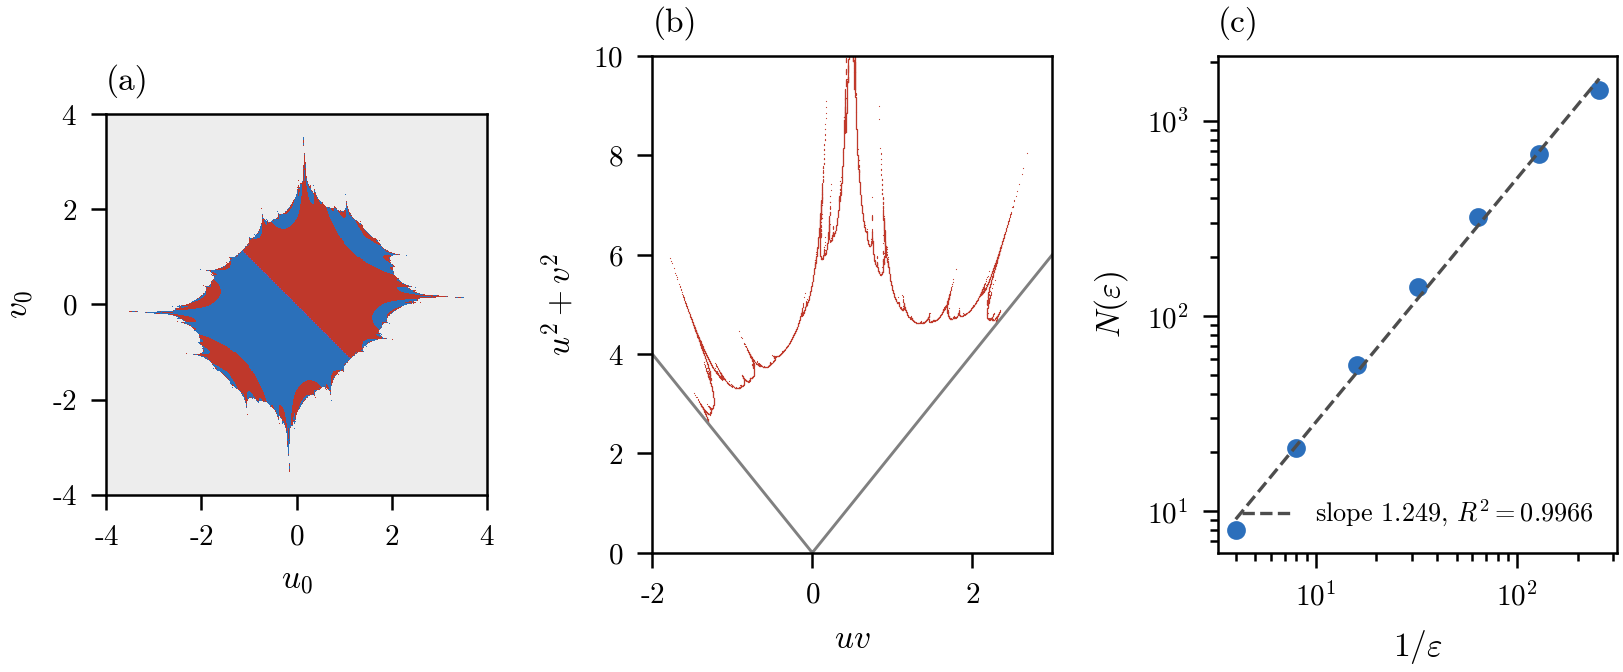
\includegraphics[width=\linewidth]{fig_reproduction.png}
  \caption{Deterministic reproduction. (a) Outcome of GD on $[-4,4]^2$: red and blue converge to $+(m,m)$ and $-(m,m)$, gray escapes. (b) Boundary of the convergence region of the projected map in the coordinates $(uv,\,u^2+v^2)$; the gray lines are $u^2+v^2=2|uv|$. (c) Box counting for (b), with slope $1.249$.}
  \label{fig:repro}
\end{figure}

\section{Small noise near the boundary}

Figure~\ref{fig:windows} shows the outcome probabilities in $W_1$ for step noise and SGD. With noise, the sharp interface of deterministic GD turns into a band of initializations whose outcome is random, and the thin filaments of the boundary disappear first. The majority outcome differs from that of deterministic GD on only $0.1$--$3.9\%$ of the cells in each window, and the fraction of initializations that do not escape changes by at most $0.014$. In this sense noise blurs the boundary but hardly moves it.

\begin{figure}[!htbp]
  \centering
  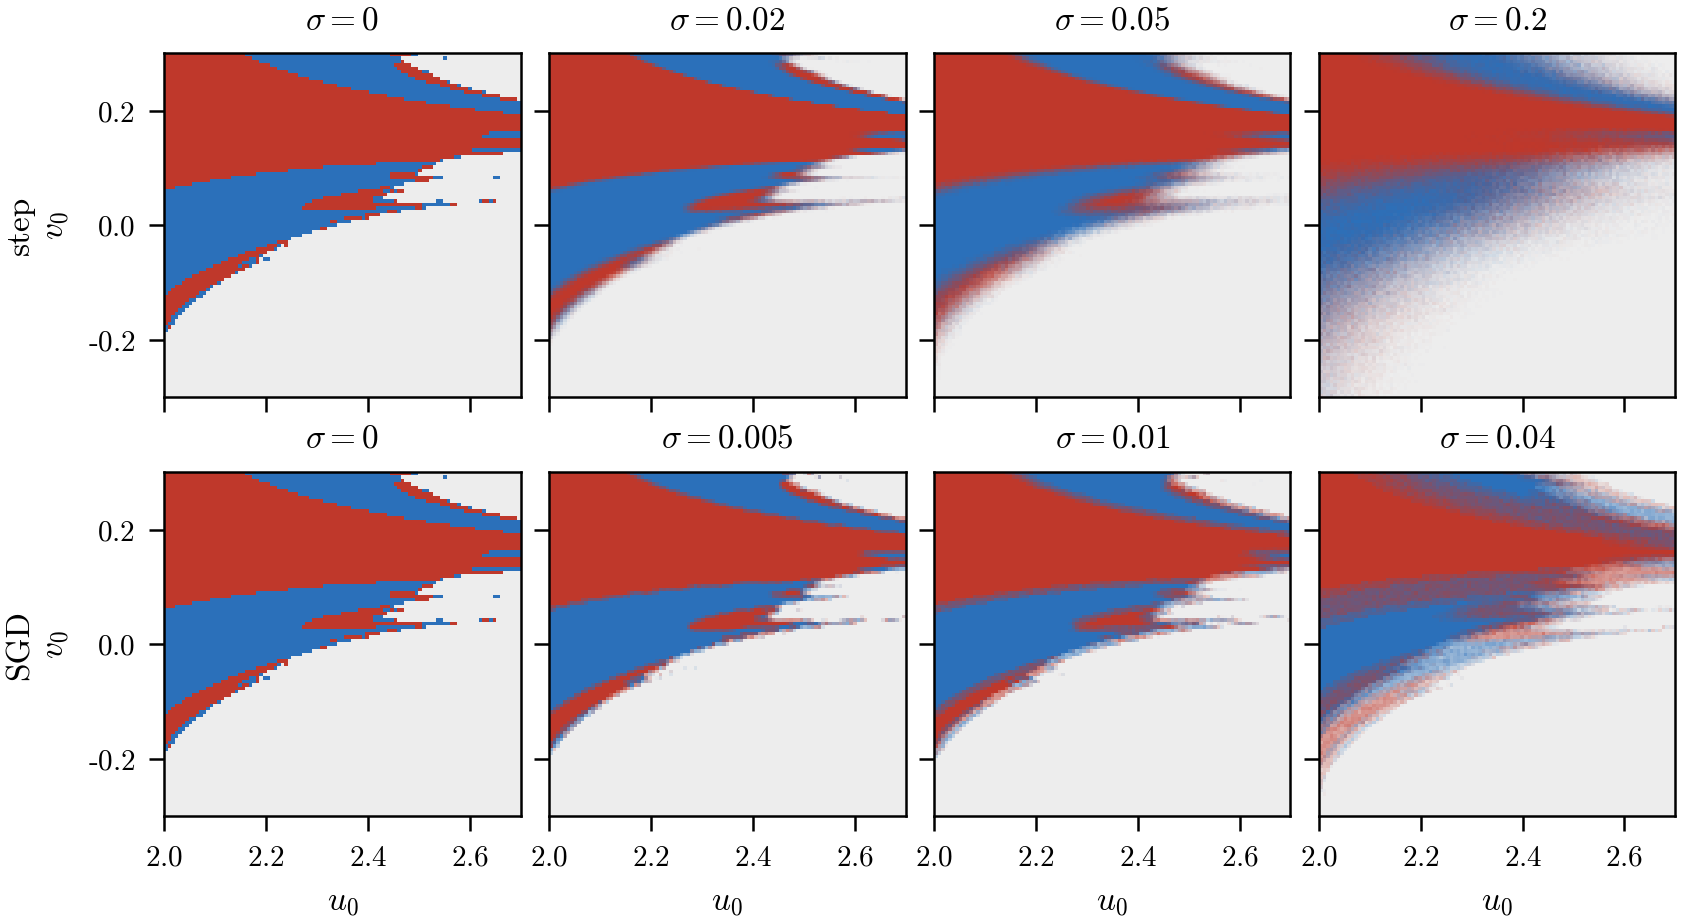
\includegraphics[width=0.92\linewidth]{fig_window_maps.png}
  \caption{Outcome probabilities in $W_1$ for step noise (top) and SGD (bottom). The color intensity of red and blue gives the probabilities of the two minimizers, and gray the probability of escape.}
  \label{fig:windows}
\end{figure}

Both uncertain fractions follow power laws $\sigma^{\beta}$ over one to two decades of $\sigma$ (Figure~\ref{fig:scaling}, $R^2\geq0.998$). The fitted exponents are listed in Table~\ref{tab:exponents} together with the deterministic uncertainty exponents. Two observations stand out. First, all noise exponents are of the same order as $2-D$, but they are not equal to it, and they depend on the noise model and the window. Second, they differ systematically between the two quantities: for escape the exponents are mostly larger than $2-D$ ($0.73$--$0.85$ versus $0.74$), while for minimizer selection they are at or below it ($0.63$--$0.72$ versus $0.71$--$0.72$). Selection therefore becomes uncertain at smaller noise levels than escape does.

\begin{table}[!htbp]
  \centering
  \caption{Exponents $\beta$ of the uncertain fractions as functions of the noise level $\sigma$, with standard errors of the least-squares fit. The last row gives the uncertainty exponent $\alpha$ of deterministic GD as a function of the perturbation size $\varepsilon$.}
  \label{tab:exponents}
  \begin{tabular}{lcccc}
    \toprule
    & \multicolumn{2}{c}{escape} & \multicolumn{2}{c}{selection} \\
    \cmidrule(lr){2-3}\cmidrule(lr){4-5}
    & $W_1$ & $W_2$ & $W_1$ & $W_2$ \\
    \midrule
    step noise     & $0.85\pm0.01$ & $0.73\pm0.01$ & $0.64\pm0.01$ & $0.63\pm0.01$ \\
    SGD            & $0.80\pm0.02$ & $0.82\pm0.02$ & $0.69\pm0.01$ & $0.65\pm0.01$ \\
    additive noise & $0.83\pm0.01$ & $0.85\pm0.01$ & $0.72\pm0.002$ & $0.65\pm0.02$ \\
    \midrule
    deterministic GD, $\alpha=2-D$ & $0.74\pm0.01$ & $0.74\pm0.005$ & $0.72\pm0.01$ & $0.71\pm0.01$ \\
    \bottomrule
  \end{tabular}
\end{table}

\begin{figure}[!htbp]
  \centering
  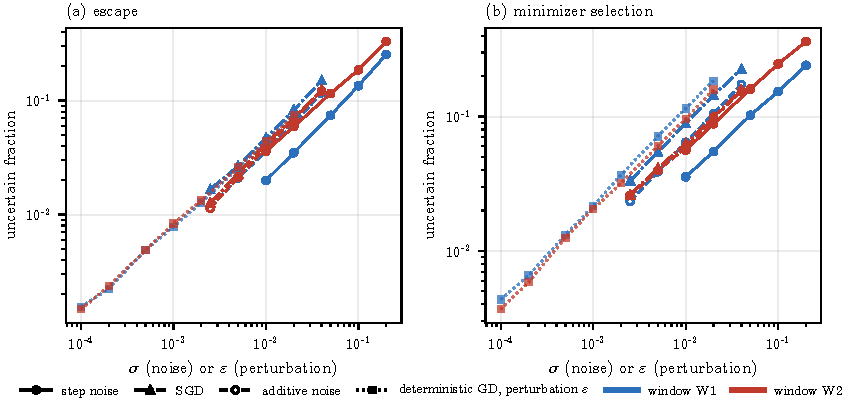
\includegraphics[width=0.95\linewidth]{fig_scaling.pdf}
  \caption{Fraction of uncertain initializations against the noise level $\sigma$, or the perturbation size $\varepsilon$ for deterministic GD, on logarithmic axes. (a) Escape. (b) Minimizer selection.}
  \label{fig:scaling}
\end{figure}

\section{Larger noise}

Over the whole domain, increasing the noise produces a qualitative change that is different for each noise model (Figures~\ref{fig:global} and~\ref{fig:globalcurves}).

With step noise the convergence region grows, from $20.9\%$ of the domain without noise to $25.1\%$ at $\sigma=0.8$, and every surviving run still converges to a minimizer, since the minimizers remain fixed points of each random step.

With SGD the change happens at a threshold. Up to $\sigma=0.2$, $99.7\%$ of surviving runs end close to a minimizer, but at $\sigma=0.4$ only $57\%$ do. For $\sigma>y-\lambda=0.3$ the sample loss $L_-$ has $y-\sigma<\lambda$, so its only minimizer is the origin, and the iterates are repeatedly pulled toward the saddle point between the two basins.

With isotropic noise at $\sigma=0.2$, the selected minimizer is uncertain on essentially the whole surviving region, and $14\%$ of surviving runs end near neither minimizer.

\begin{figure}[!htbp]
  \centering
  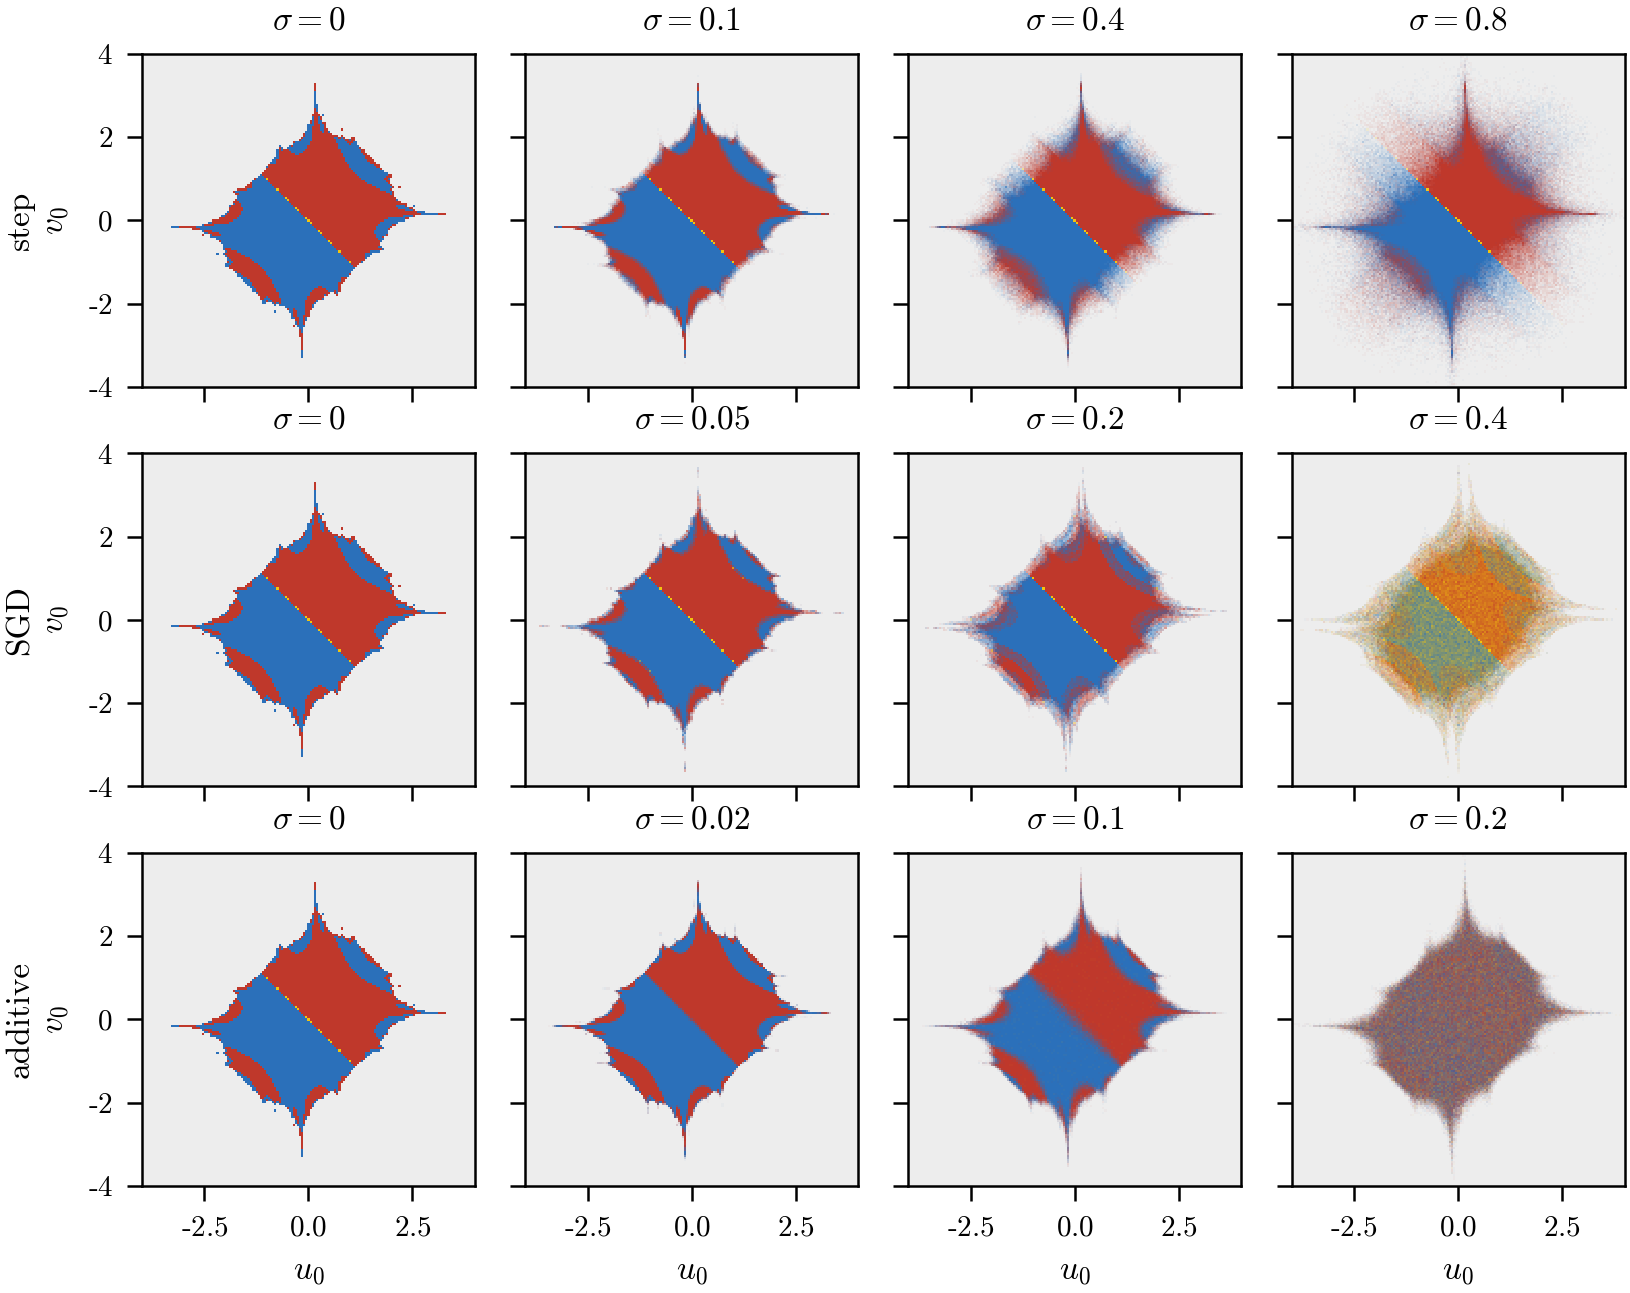
\includegraphics[width=0.86\linewidth]{fig_global.png}
  \caption{Outcome probabilities on $[-4,4]^2$ for increasing noise. Rows: step noise, SGD, additive noise. Colors as in Figure~\ref{fig:windows}; gold marks surviving runs that end near neither minimizer.}
  \label{fig:global}
\end{figure}

\begin{figure}[!htbp]
  \centering
  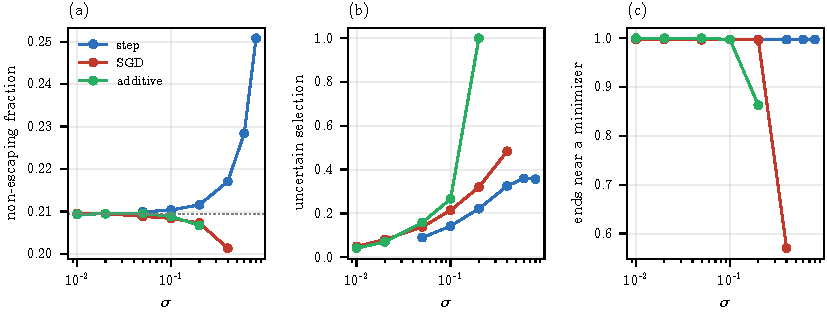
\includegraphics[width=\linewidth]{fig_global_curves.pdf}
  \caption{Whole-domain summaries against $\sigma$. (a) Fraction of initializations that do not escape; the dotted line is deterministic GD. (b) Fraction of the surviving region on which the selected minimizer is uncertain. (c) Fraction of surviving runs that end close to a minimizer.}
  \label{fig:globalcurves}
\end{figure}

\section{Controls}

With step noise at $\sigma=0.1$ and $n=64$, the uncertain escape fraction in $W_1$ is $0.134$ on an $81\times81$ grid and $0.135$ on a $161\times161$ grid, and $0.136$ when the horizon is doubled to $T=400$. Figure~\ref{fig:coupling} shows why we use probabilities rather than single runs. If all initializations share one noise sequence, the boundary stays sharp. If each initialization receives its own noise sequence, the map is dominated by isolated speckle, and its interface is about four times longer ($0.059$ versus $0.016$ of the cells). Box counting on such a map measures the sampling noise and not the geometry of the boundary; an earlier version of this analysis made exactly this error.

\begin{figure}[!htbp]
  \centering
  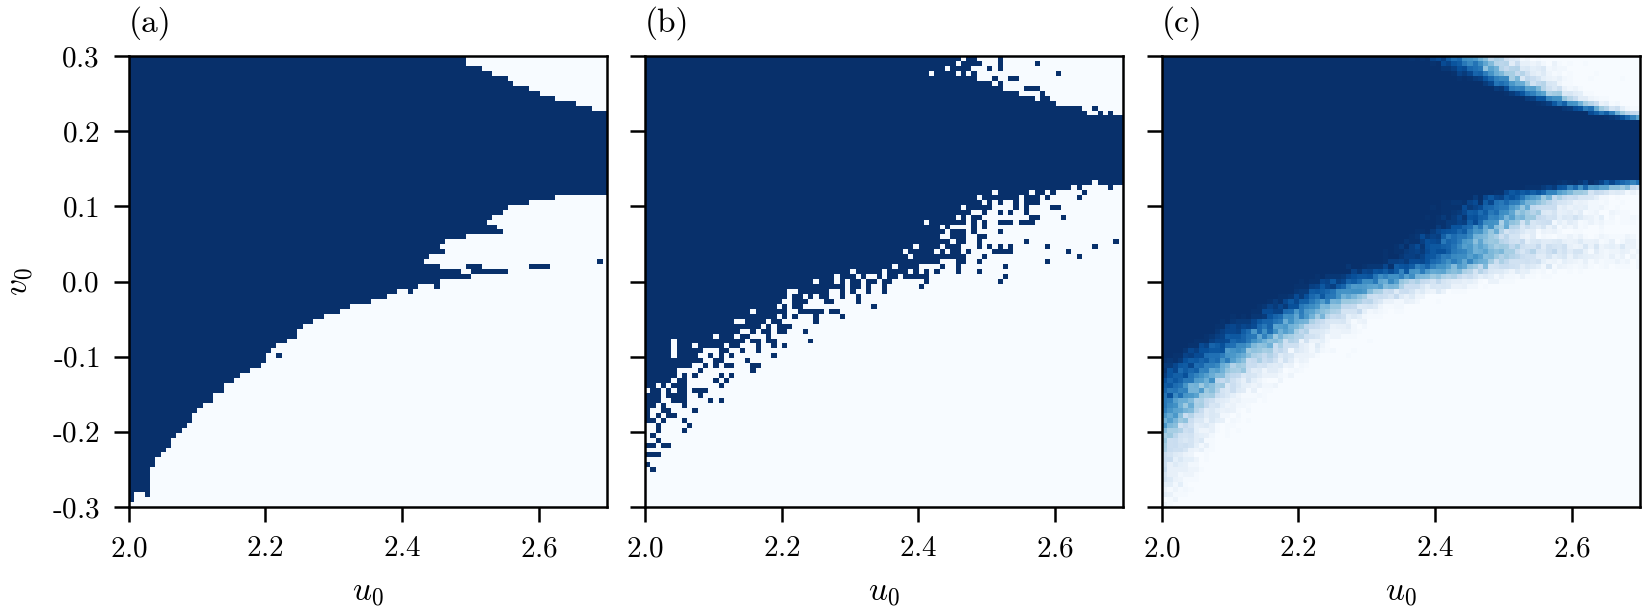
\includegraphics[width=\linewidth]{fig_coupling.png}
  \caption{Step noise with $\sigma=0.1$ in $W_1$. (a) One noise sequence shared by all initializations. (b) An independent noise sequence for each initialization. (c) Probability of not escaping, from $n=64$ runs per initialization.}
  \label{fig:coupling}
\end{figure}

\section{Discussion}

If the noise acted only as a single random displacement of the initialization of size proportional to $\sigma$, one would expect the uncertain fractions to scale like $\sigma^{2-D}$. The exponents we measure are of this order, which is consistent with the fractal boundary controlling how outcomes become uncertain. They do not, however, agree with $2-D$ exactly, and they deviate in opposite directions for escape and for selection. One possible explanation is that noise injected at every step interacts differently with the two parts of the boundary, but we have not tested this. This suggests a few questions that may be suitable for a mathematical treatment:
\begin{enumerate}
  \item Can the noise exponents be derived from the dimension of the boundary and the expansion rate of the GD map?
  \item Why is minimizer selection more sensitive to noise than convergence?
  \item Can the growth of the convergence region under random step sizes be explained using the critical step size of Theorem~1 in~\cite{liang2026}?
\end{enumerate}
Sohl-Dickstein~\cite{sohldickstein2024} observed that fractal trainability boundaries survive minibatch training. Our shared-noise control is consistent with this, since a fixed sequence of minibatches corresponds to a single shared noise path, for which the boundary remains sharp.

\paragraph{Limitations.} Surviving for $T$ steps is not the same as converging, and under persistent noise (SGD and additive noise) the iterates fluctuate around a minimizer rather than converging to it. The results are based on two windows, a particular choice of the thresholds $0.1$ and $0.9$, and $96$ runs per initialization near the boundary and $32$ over the whole domain. Only the scalar case is considered; matrix factorization and minibatch training of real models are not tested.

\begin{thebibliography}{9}
\bibitem{grebogi1983}
C.~Grebogi, S.~W. McDonald, E.~Ott, and J.~A. Yorke.
\newblock Final state sensitivity: an obstruction to predictability.
\newblock \emph{Physics Letters A}, 99(9):415--418, 1983.

\bibitem{liang2026}
S.~Liang and G.~Mont\'ufar.
\newblock Gradient descent with large step sizes: chaos and fractal convergence region.
\newblock In \emph{International Conference on Learning Representations (ICLR)}, 2026.
\newblock arXiv:2509.25351.

\bibitem{nieto2021}
A.~R. Nieto, J.~M. Seoane, and M.~A.~F. Sanju\'an.
\newblock Final state sensitivity in noisy chaotic scattering.
\newblock \emph{Chaos, Solitons \& Fractals}, 150:111181, 2021.

\bibitem{sohldickstein2024}
J.~Sohl-Dickstein.
\newblock The boundary of neural network trainability is fractal.
\newblock arXiv:2402.06184, 2024.
\end{thebibliography}

\end{document}
